\documentclass[a4paper,11pt]{article}
\usepackage[spanish]{babel}
\usepackage[utf8]{inputenc}

% Configuración páginas
\usepackage{vmargin}							% Márgenes

\usepackage{sectsty}							% Fuente de los títulos
\allsectionsfont{\normalfont \Large \scshape}

\usepackage{graphicx}							% Imágenes
\graphicspath{{images/}}

\usepackage{tabularx}							% Otras tablas
\usepackage{listliketab}						% Tratar indentacion distas como tablas

\usepackage{mathtools}							% Matematicas
\newcommand\numberthis{							% numeración en align*
	\addtocounter{equation}{1}\tag{\theequation}
}

% Configuración del título
\newcommand{\horrule}[1]{\rule{\linewidth}{#1}} 	% Horizontal rule

\title{
	\vspace{-25pt}
	\normalfont \Large \textsc{
		Modelos de Investigación Operativa,
        Ingeniería Informática\\
        Universidad de Valladolid
	}\\[10pt]
	\horrule{1pt}\\[10pt]
	\huge \textbf{
		Práctica 8
	}\\
	\horrule{1pt}
}
\author{
	\normalfont \Large Daniel González Alonso
}
\date{
	\normalfont \large \today
}

%%%%%%%%%%%%%%%%%%%%%%%%%%%%%%%%%%%%%%%%%%%%%%%%%%
\begin{document}
\maketitle

%%%% RESUMEN %%%%
\begin{abstract}
	En este documento se describen los problemas y los resultados obtenidos de la práctica 8 del tema 3 de la asignatura Modelos de Investigación Operativa de Ingeniería Informática, Universidad de Valladolid.
\end{abstract}

%%%% DESARROLLO %%%%
\section{Introducción}
Esta práctica trata de problemas de P-mediana. El modelo empleado para resolver estos problemas es el siguiente:

\begin{align*}\numberthis
   	&\textrm{Minimizar }	&& z = \sum_{i=1}^{m}{\sum_{j=1}^{n}{h_i \cdot d_{i,j} \cdot y_{i,j}}}	&& \\
   	&\textrm{Sujeto a }		&& \sum_{j=1}^{n}{y_{i,j}} = 1 					&& i=1,\ldots,m \\
    &						&& y_{i,j} \leq x_j								&& i=1,\ldots,m \ \ j=1,\ldots,n \\
    &						&& \sum_{j=1}^{n}{x_j} = P						&&				\\
	&						&& x_{j} \in \{0,1\}							&& j=1,\ldots,n \\
	&						&& y_{i,j} \in \{0,1\}							&& i=1,\ldots,m \ \ j=1,\ldots,n
\end{align*}

Donde ${h_i}$ representa la demanda del punto ${i}$, ${d_{i,j}}$ contiene las distancias del punto ${i}$ al punto ${j}$, ${P}$ es el número de instalaciones que van a ser abiertas, ${x_j}$ es la variable de decisión que indica 1 si una instalación va a ser abierta en el punto ${j}$ o 0 en caso contrario y por último ${y_{i,j}}$ es la variable de decisión que dice si el punto ${j}$ queda asignado a la instalación ${i}$ en caso de valer 1 o 0 en caso contrario.


%%%%%%%%%%%%%%%%%%%%%%%%%%%%%%%%%%%%%%%%%%%%%%%%%%%%%%
\newpage
\section{Desarrollo}
Para esta práctica se nos pide resolver el problema de P-mediana de forma exacta y de forma heurística (método greedy obligatorio, método de búsqueda local voluntario), para los archivos de datos \texttt{data/coordenadas\_15.dat}, \texttt{data/coordenadas\_30.dat} y \texttt{data/coordenadas\_100.dat}, con valores de ${p}$ desde 1 hasta 10. De forma opcional se nos pide extraer los gráficos IVE de las soluciones obtenidas.\\

Este problema se encuentra resuelto mediante \textit{Xpress Mosel} en los ficheros de datos <nombres> (el nombre indica el fichero de datos empleado).\\

Para resolver esta practica en cada uno de los ficheros lo primero que se hizo fue cargar los datos. El formato de los datos \textit{coordenadas} es el siguiente:

\storestyleof{itemize}
\begin{listliketab}
    \begin{tabular}{Lll}
\textbullet	& ${n}$				& Número de puntos (de servicio y de demanda)	\\
\textbullet	& ${i=1,\ldots,n}$	& El índice, su coordenada x, su coordenada y su demanda	\\
    \end{tabular}
\end{listliketab}

La primero que se hizo fue resolver de \textbf{forma exacta} con los distintos conjuntos de datos mediante \textit{Xpress Mosel}. Debido a que este problema excede el numero de restricciones de la versión de estudiante, este problema se resolvió en los ficheros de forma separada en los ordenadores de clase mediante los ficheros \texttt{p\_mediana\_exacta\_15.mos}, \texttt{p\_mediana\_exacta\_30.mos} y \texttt{p\_mediana\_exacta\_100.mos}. Para el calculo de las distancias, antes de empezar el modelo se calcula la matriz ${d_{i,j}}$ a partir de las coordenadas dadas mediante la distancia euclídea redondeada al entero más cercano.\\

Lo siguiente que hice fue el \textbf{Algoritmo Greedy} para la P-Mediana. Para este algoritmo se llevaron a cabo las siguiente etapas:

\begin{enumerate}
\item Se inicializa todos los valores de la solución ${X_j}$ a 0 y el contador de instalaciones asignadas ${k=0}$.
\item Para cada punto ${j}$ que no esté en la solución se calcula el valor ${Z_{j}^{k}}$ mediante la siguiente ecuación:

\begin{equation}
Z_{j}^{k} = \sum_{i}{h_{i}\times d(i,j \cup X_{k-1})}
\end{equation}

Donde el valor de ${d(i,j \cup X_{k-1})}$ representa la distancia mínima entre el punto de demanda ${i}$ y el punto más cercano después de añadir a la solución el punto de servicio ${j}$. En mi caso para calcular este valor lo que hize fue mantener un vector con las distancias mínimas a cada punto de demanda en las iteraciones anteriores (iniciado con todos los valores a infinito) y calcular el minimo entre el posible punto de demanda ${j}$ (${d_{i,j}}$) y el valor actual en ese vector.

\item Se busca el punto ${j_{k}^{*}}$ que minimiza ${Z_{j}^{k}}$. Para este paso cree una función llamada \texttt{getIndiceMinimo} que dado un array devuelve el indice del elemento con el menor valor del array.

\item Añadimos el valor anterior ${j_{k}^{*}}$ a la solución y aumentamos el contador de instalaciones asignadas ${k}$. Además actualizamos el vector con las distancias mínimas tras añadir este valor a la solución.

\item Si ${k}$ es menor que ${p}$ volvemos al paso 2, si no ya tenemos nuestra solución greedy.
\end{enumerate}

La solución greedy se encuentra resuelta mediante \textit{Xpress Mosel} en los archivos \texttt{\\p\_mediana\_greedy\_15.mos}, \texttt{p\_mediana\_greedy\_30.mos} y \texttt{p\_mediana\_greedy\_100.mos}.\\

Por último también hice el trabajo voluntario de hacer el \textbf{método greedy con búsqueda local}. El método de búsqueda local parte de una solución ya dada, en nuestro caso el resultado del algoritmo Greedy, y realiza un descenso hasta obtener un valor óptimo local. En mi caso se empleo un heurística de intercambios, en la cual se prueba a intercambiar un valor de ${j}$ que se encuentra en la solución por otro que no está. En caso de que este intercambio produzca una mejora en la distancia total, se realiza el intercambio y se vuelve a hacer el método de búsqueda local hasta que no se mejore. El método de búsqueda local se encuentra implementado mediante \textit{Xpress Mosel} en los archivos \texttt{\\p\_mediana\_greedy\_busqueda\_local\_15.mos}, \texttt{p\_mediana\_greedy\_busqueda\_local\_30.mos} y \texttt{p\_mediana\_greedy\_busqueda\_local\_100.mos}.\\

\newpage
\section{Resultados}

\begin{itemize}
\item Resultados obtenidos para \texttt{coordenadas\_15.dat}:

\begin{table}[!htbp]
\label{results_15}
\centering
\begin{tabularx}{\textwidth}{|X|X|X|X|}
\hline
Valor de ${P}$	& Método Exacto	& Algoritmo Greedy & Algoritmo Greedy con búsqueda local \\ \hline
1	& 1331310	& 1331306	& 1331306	\\ \hline
2	& 868883	& 899890	& 868883	\\ \hline
3	& 643399	& 667582	& 643399	\\ \hline
4	& 514063	& 559924	& 514063	\\ \hline
5	& 400066	& 454850	& 400066	\\ \hline
6	& 327956	& 365942	& 327956	\\ \hline
7	& 268260	& 281991	& 268786	\\ \hline
8	& 209090	& 213767	& 209090	\\ \hline
9	& 163694	& 168371	& 163694	\\ \hline
10	& 124955	& 129632	& 124955	\\ \hline
\end{tabularx}
\end{table}

\item Resultados obtenidos para \texttt{coordenadas\_30.dat}:

\begin{table}[!htbp]
\label{results_30}
\centering
\begin{tabularx}{\textwidth}{|X|X|X|X|}
\hline
Valor de ${P}$	& Método Exacto	& Algoritmo Greedy & Algoritmo Greedy con búsqueda local \\ \hline
1	& 2720260	& 2720256	& 2720256	\\ \hline
2	& 1972150	& 2170429	& 1972149	\\ \hline
3	& 1594790	& 1710294	& 1594788	\\ \hline
4	& 1328110	& 1406866	& 1406866	\\ \hline
5	& 1122130	& 1212708	& 1122125	\\ \hline
6	& 974818	& 1032328	& 974818	\\ \hline
7	& 852906	& 931177	& 974818	\\ \hline
8	& 753969	& 830299	& 753969	\\ \hline
9	& 685166	& 742191	& 697254	\\ \hline
10	& 617845	& 672541	& 628451	\\ \hline
\end{tabularx}
\end{table}

\item Resultados obtenidos para \texttt{coordenadas\_100.dat}:

\begin{table}[!htbp]
\label{results_100}
\centering
\begin{tabularx}{\textwidth}{|X|X|X|X|}
\hline
Valor de ${P}$	& Método Exacto	& Algoritmo Greedy & Algoritmo Greedy con búsqueda local \\ \hline
1	& 9108490	& 9108490	& 9108490	\\ \hline
2	& 6375340	& 7054059	& 6375338	\\ \hline
3	& 5206490	& 5663114	& 5323818	\\ \hline
4	& 4281110	& 4802205	& 4281107	\\ \hline
5	& 3728220	& 4154751	& 3728221	\\ \hline
6	& 3363510	& 3526319	& 3407864	\\ \hline
7	& 3071410	& 3142797	& 3071405	\\ \hline
8	& 2779500	& 2852233	& 2779500	\\ \hline
9	& 2583750	& 2648007	& 2583749	\\ \hline
10	& 2392640	& 2474262	& 2392643	\\ \hline
\end{tabularx}
\end{table}
\end{itemize}

\newpage
A continuación también se muestran unos de los gráficos IVE obtenidos comparando la solución del algoritmo Greedy con el algoritmo greedy con búsqueda local para el fichero de coordenadas 100.

\begin{table}[!htbp]
\label{images_100}
\centering
\begin{tabularx}{\textwidth}{|p{1cm}|X|X|}
\hline
Valor de P	& Solución Greedy	& Solución Greedy con búsqueda local	\\ \hline
2 & 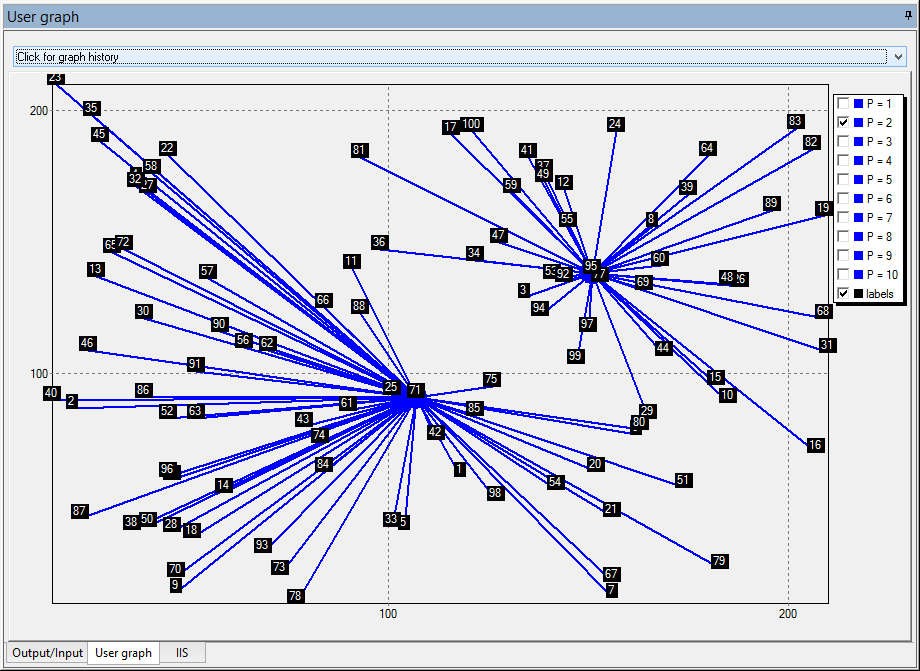
\includegraphics[width=6.5cm, height=4cm]{images/greedy_100_p2.png}	& 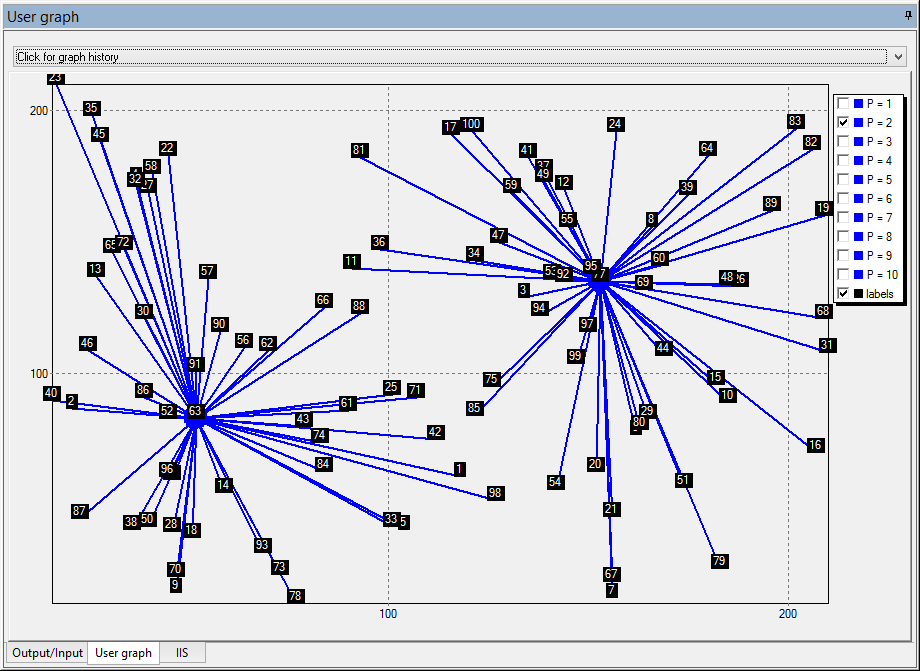
\includegraphics[width=6.5cm, height=4cm]{images/greedy_busqueda_local_100_p2.png}	\\ \hline
4 & 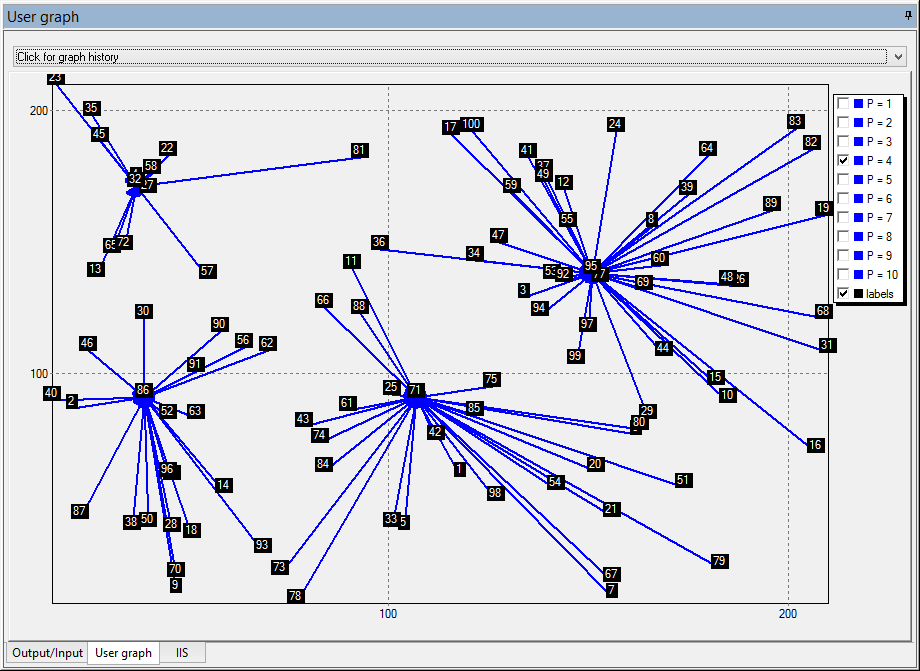
\includegraphics[width=6.5cm, height=4cm]{images/greedy_100_p4.png}	& 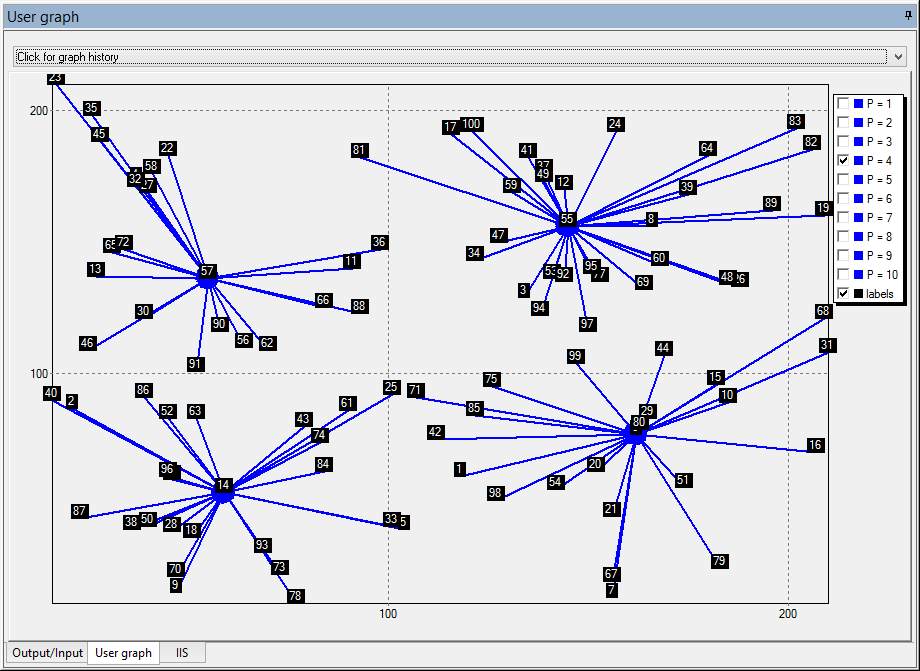
\includegraphics[width=6.5cm, height=4cm]{images/greedy_busqueda_local_100_p4.png}	\\ \hline
6 & 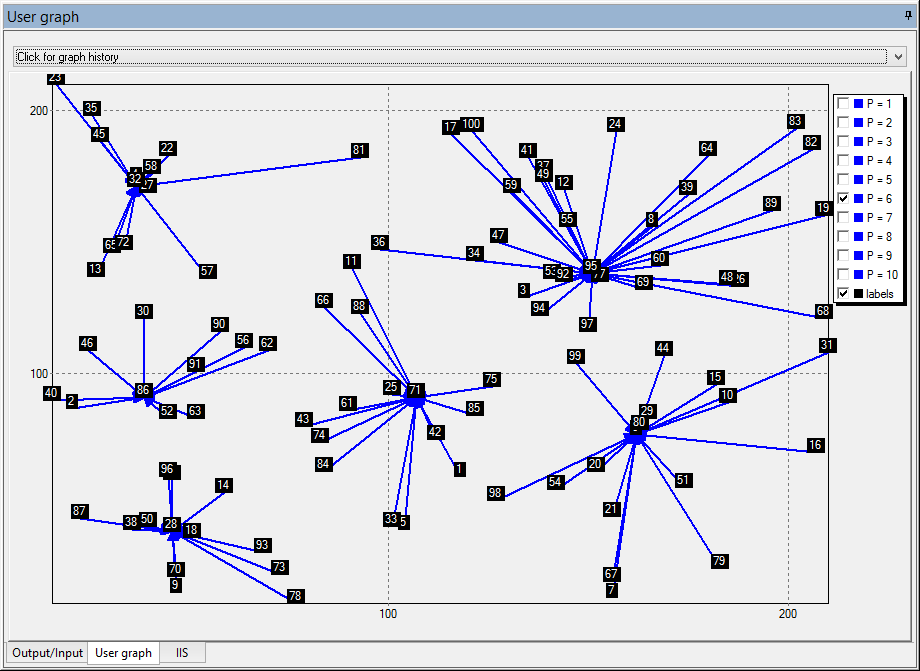
\includegraphics[width=6.5cm, height=4cm]{images/greedy_100_p6.png}	& 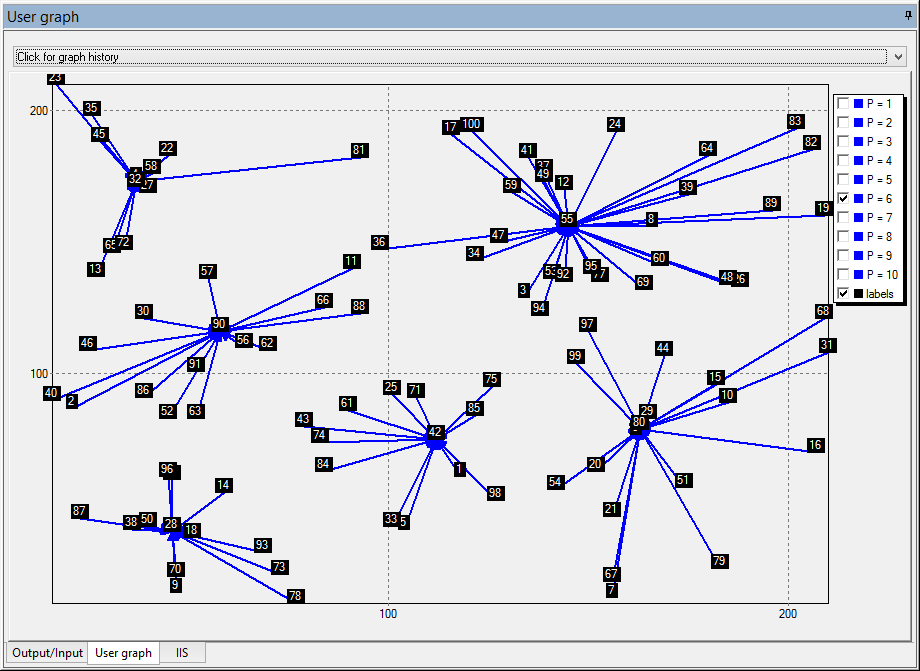
\includegraphics[width=6.5cm, height=4cm]{images/greedy_busqueda_local_100_p6.png}	\\ \hline
8 & 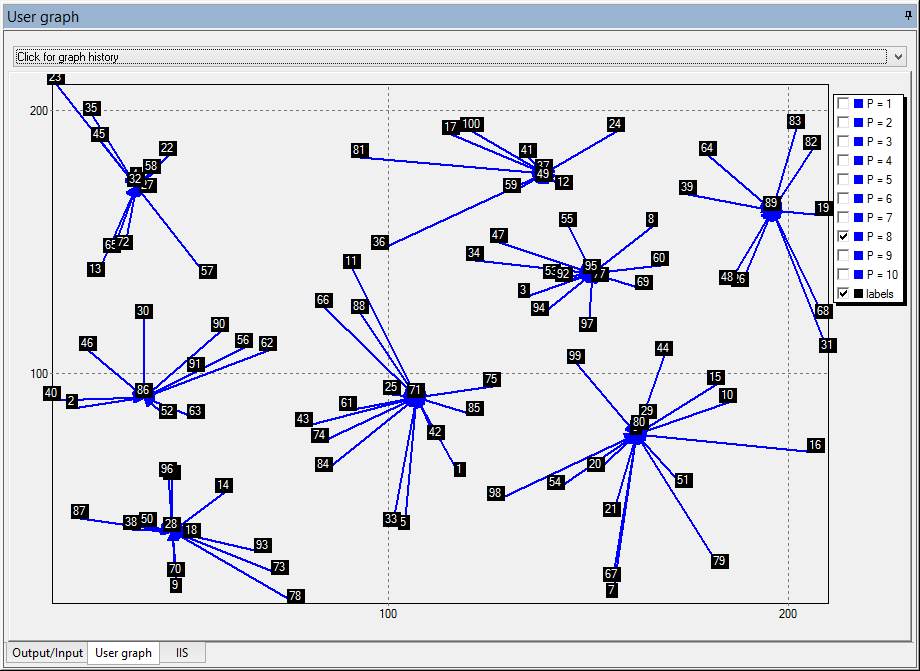
\includegraphics[width=6.5cm, height=4cm]{images/greedy_100_p8.png}	& 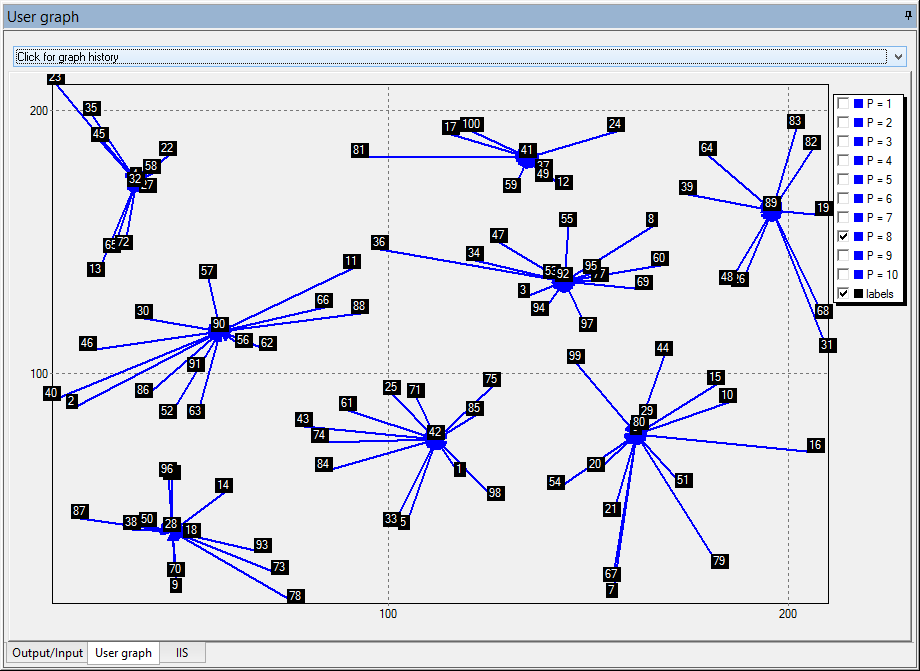
\includegraphics[width=6.5cm, height=4cm]{images/greedy_busqueda_local_100_p8.png}	\\ \hline
10 & 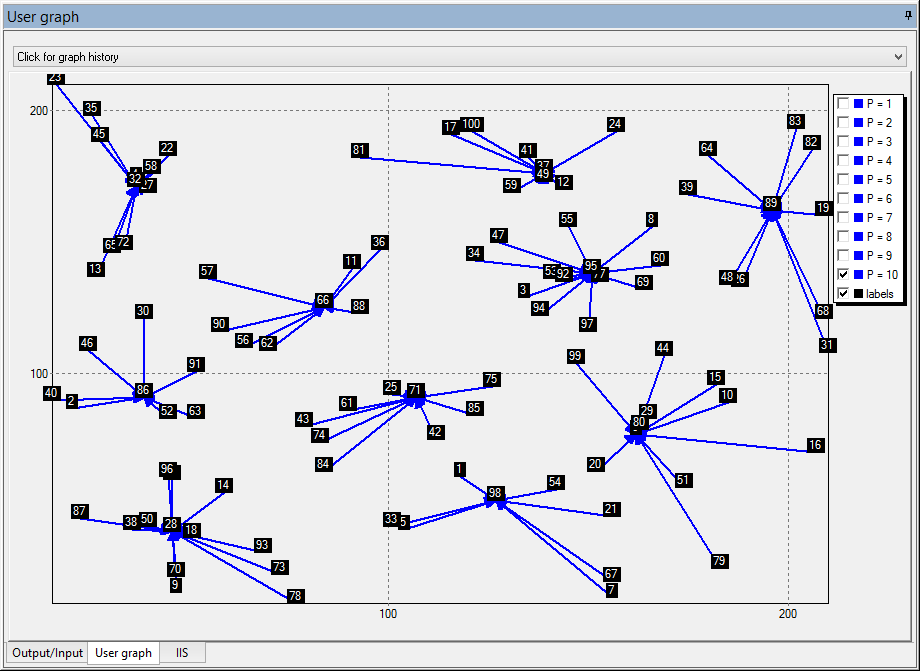
\includegraphics[width=6.5cm, height=4cm]{images/greedy_100_p10.png}	& 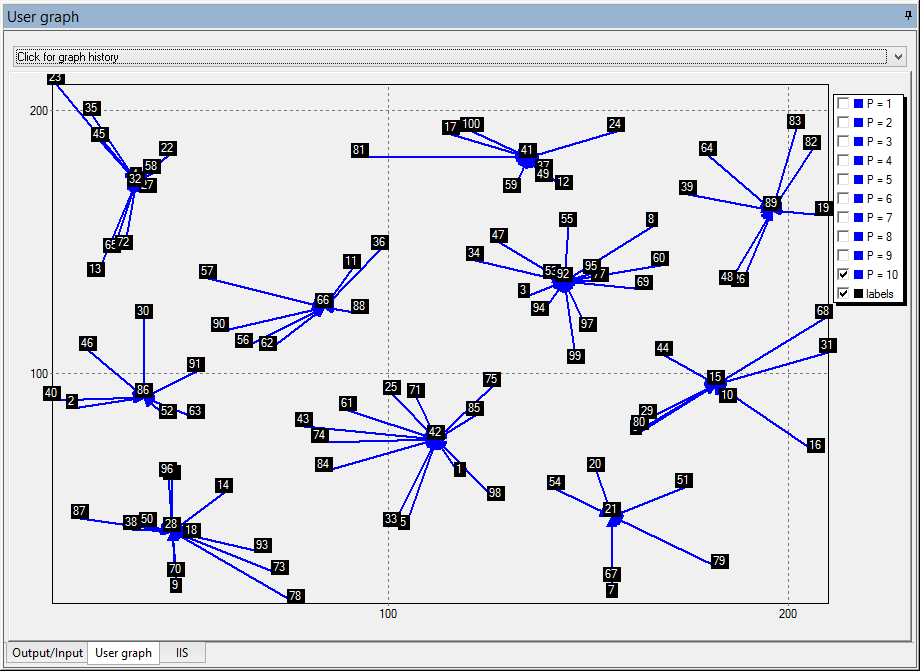
\includegraphics[width=6.5cm, height=4cm]{images/greedy_busqueda_local_100_p10.png}	\\ \hline
\end{tabularx}
\end{table}
\end{document}
